\documentclass{standalone}
\usepackage{tikz}
\usepackage{siunitx}
\usetikzlibrary{shapes, patterns, decorations.pathmorphing}

\begin{document}
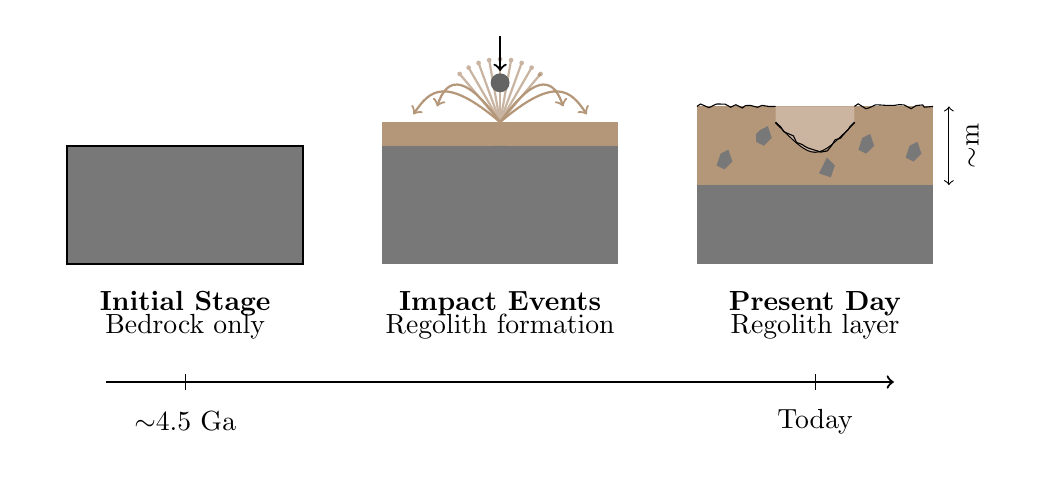
\begin{tikzpicture}

% Define colors
\definecolor{bedrock}{RGB}{120, 120, 120}
\definecolor{regolith}{RGB}{180, 150, 120}
\definecolor{meteorite}{RGB}{100, 100, 100}
\definecolor{plume}{RGB}{200, 180, 160}

% Initial Stage - Only Bedrock
\begin{scope}[xshift=0cm]
    % Bedrock
    \fill[bedrock] (0,0) rectangle (3,1.5);
    \draw[thick] (0,0) rectangle (3,1.5);
    
    % Label
    \node at (1.5,-0.5) {\textbf{Initial Stage}};
    \node at (1.5,-0.8) {Bedrock only};
\end{scope}

% Intermediate Stage - Impact Event
\begin{scope}[xshift=4cm]
    % Bedrock
    \fill[bedrock] (0,0) rectangle (3,1.5);
    
    % Thin regolith layer
    \fill[regolith] (0,1.5) rectangle (3,1.8);
    
    % Impact crater (simplified)
    \fill[bedrock] (1.2,1.2) -- (1.8,1.2) -- (1.6,1.5) -- (1.4,1.5) -- cycle;
    
    % Ejecta plume - extended and more realistic
    \foreach \angle in {50,60,70,80,90,100,110,120,130} {
        \draw[thick, plume] (1.5,1.8) -- +(\angle:0.8);
        \fill[plume] (1.5,1.8) +(\angle:0.8) circle (0.03);
    }
    
    % Parabolic falling particles from plume
    % Left trajectory
    \draw[thick, regolith, ->] (1.5,1.8) .. controls (0.8,2.4) and (0.6,2.2) .. (0.4,1.9);
    
    % Left-center trajectory
    \draw[thick, regolith, ->] (1.5,1.8) .. controls (1.0,2.5) and (0.8,2.3) .. (0.7,2.0);
    
    % Right-center trajectory
    \draw[thick, regolith, ->] (1.5,1.8) .. controls (2.0,2.5) and (2.2,2.3) .. (2.3,2.0);
    \fill[regolith] (2.0,2.4) circle (0.025);
    \fill[regolith] (2.2,2.2) circle (0.025);
    
    % Right trajectory
    \draw[thick, regolith, ->] (1.5,1.8) .. controls (2.2,2.4) and (2.4,2.2) .. (2.6,1.9);

    % Meteorite - made larger and more visible
    \fill[meteorite] (1.5,2.3) circle (0.12);
    \draw[thick, ->] (1.5,2.9) -- (1.5,2.45);
    
    % Label
    \node at (1.5,-0.5) {\textbf{Impact Events}};
    \node at (1.5,-0.8) {Regolith formation};
\end{scope}

% Current Stage - Thick Regolith Layer
\begin{scope}[xshift=8cm]
    % Bedrock
    \fill[bedrock] (0,0) rectangle (3,1);
    
    % Thick regolith layer with rock fragments
    \fill[regolith] (0,1) rectangle (3,2);
    
    % Rock fragments in regolith - more realistic irregular shapes
    \fill[bedrock] (0.25,1.25) -- (0.35,1.2) -- (0.45,1.3) -- (0.4,1.45) -- (0.3,1.4) -- cycle;
    \fill[bedrock] (0.75,1.55) -- (0.85,1.5) -- (0.95,1.6) -- (0.9,1.75) -- (0.8,1.7) -- (0.75,1.65) -- cycle;
    \fill[bedrock] (1.55,1.15) -- (1.7,1.1) -- (1.75,1.25) -- (1.65,1.35) -- (1.6,1.25) -- cycle;
    \fill[bedrock] (2.05,1.45) -- (2.15,1.4) -- (2.25,1.5) -- (2.2,1.65) -- (2.1,1.6) -- cycle;
    \fill[bedrock] (2.65,1.35) -- (2.75,1.3) -- (2.85,1.4) -- (2.8,1.55) -- (2.7,1.5) -- cycle;
    
    % Crater with less regolith - made larger and regolith follows crater shape
    \draw[thick] (1.0,1.8) .. controls (1.5,1.3) .. (2.0,1.8);
    \fill[regolith!70] (1.0,1.8) .. controls (1.5,1.3) .. (2.0,1.8) -- (2.0,2) -- (1.0,2) -- cycle;
    
    % Surface texture - modified to follow crater contour
    \draw[decorate, decoration={random steps, segment length=2pt, amplitude=1pt}] (0,2) -- (1.0,2);
    \draw[decorate, decoration={random steps, segment length=2pt, amplitude=1pt}] (1.0,1.8) .. controls (1.5,1.3) .. (2.0,1.8);
    \draw[decorate, decoration={random steps, segment length=2pt, amplitude=1pt}] (2.0,2) -- (3,2);
    
    % Dimension line
    \draw[<->] (3.2,1) -- (3.2,2);
    \node[rotate=90] at (3.5,1.5) {$\sim$\si{\meter}};
    
    % Label
    \node at (1.5,-0.5) {\textbf{Present Day}};
    \node at (1.5,-0.8) {Regolith layer};
\end{scope}

% Time axis
\draw[thick, ->] (+0.5,-1.5) -- (10.5,-1.5);

% Time markers
\draw (1.5,-1.4) -- (1.5,-1.6);
\draw (9.5,-1.4) -- (9.5,-1.6);  % Changed from 11.5 to 9.5

\node at (1.5,-2) {$\sim$4.5 Ga};
\node at (9.5,-2) {Today};  % Changed from 11.5 to 9.5

% Add invisible bounding box for extra whitespace
\path (-0.5,-2.5) rectangle (12,3);

\end{tikzpicture}
\end{document}